\documentclass[10pt]{article}
\usepackage[utf8]{inputenc}
\usepackage{natbib}
\usepackage{graphicx}
\usepackage[portuguese]{babel}

\title{IF689 - Informática Teórica}
\author{Igor Domingos da Rocha e Silva }
\date{Abril 2019}

\begin{document}

\maketitle

\section{Introdução}
Infórmatica Teórica é uma disciplina que está ligada a área da computação básica e aborda conceitos da teoria da computação, buscando determinar quais problemas podem ser computados, o quão rápidos são e a quantidade de memória que ocupam,  em um dado modelo de computação. Ela estuda problemas computacionais e as classes das linguagens que podem ser produzidas e reconhecidas por modelos computacionais simbólicos. Além disso, também faz o estudo da complexidade dos algoritmos. Alguns dispositivos conhecidos, como por exemplo, as máquinas de Turing são estudados durante essa cadeira.
\cite{livro, Cin-Wiki, if689}
\begin{figure}[h!]
\centering
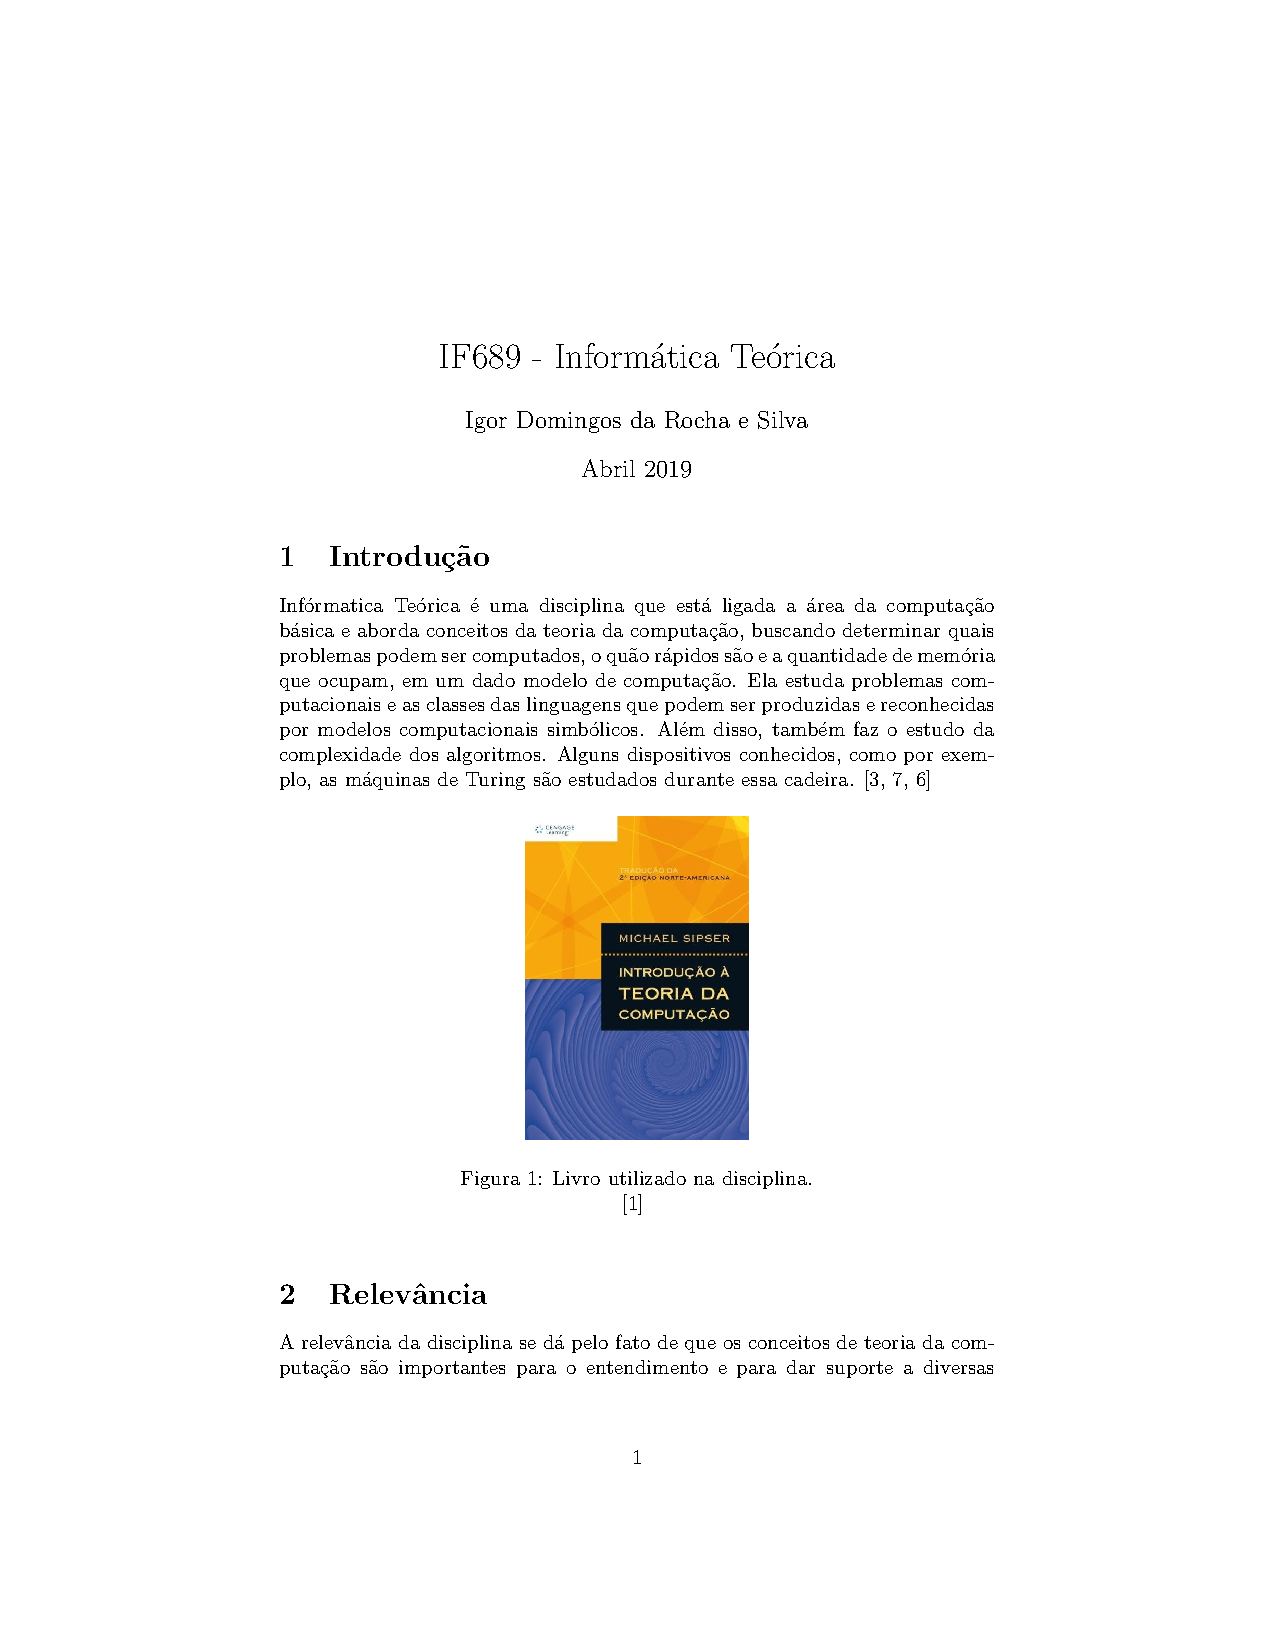
\includegraphics[scale=0.25]{idrs.jpg}
\caption{Livro utilizado na disciplina.}
\cite{img}
\label{fig:livro}
\end{figure}

\section{Relevância}
A relevância da disciplina se dá pelo fato de que os conceitos de teoria da computação são importantes para o entendimento e para dar suporte a diversas aplicações práticas da computação, tais como: análise de algoritmos (complexidade computacional), criptografia, especificação e verificação de programas, entre outros. Por esses motivos, Informática Teórica é uma cadeira presente tanto no curso de Ciência da Computação, como também no curso de Engenharia da Computação do CIn - UFPE.
\cite{relevancia}
\section{Relação com outras disciplinas}
\cite{if672, if673}
\begin{center}
\begin{tabular}{|c|l|}
\hline
Disciplina                                                                             & \multicolumn{1}{c|}{Relações}                                                                                                                                                     \\ \hline
\begin{tabular}[c]{@{}c@{}}IF - 672 \\ (Algoritmos e Estruturas de Dados)\end{tabular} & \begin{tabular}[c]{@{}l@{}}Essa disciplina estuda conceitos de \\ estruturas de dados e algoritmos e é \\ um pré-requisito para a cadeira de \\ Informática Teórica.\end{tabular} \\ \hline
\begin{tabular}[c]{@{}c@{}}IF - 673\\ (Lógica para Computação)\end{tabular}            & \begin{tabular}[c]{@{}l@{}}Essa disciplina estuda ferramentas \\ da lógica matemática e é um \\ pré-requisito para a cadeira de \\ Informática Teórica.\end{tabular}              \\ \hline
\end{tabular}
\end{center}
\bibliographystyle{plain}
\bibliography{idrs}
\end{document}
